\section{Authentication}
\label{design:authentication}
\label{design:authentication:requirements}
\label{design:authentication:solution}

\noindent Authentication consists of two steps:
\begin{enumerate}
	\item Validating
	\item Confirmation
\end{enumerate}
Validation is needed to ensure privacy. Confirmation is a requirement as error prevention, in case validation with a wrong identity is performed.
As stated, being able to launch a \girafapp[] as a specific guardian requires the user to interact such that the launcher knows which guardian the user represents.
As stated in \autoref{design:authentication:requirements}, privacy is required since each modelled child and guardian contains private data and therefore needs to be protected.
QR-codes were chosen as the means of authentication, as they provide some level of security.
An alternative to QR-codes could be a \emph{username-password} combination, where each user has their own username, with a private password.
However, as the launcher is developed towards being a tool usable by both guardians and children, a username-password combination is inappropriate, as it can diminish usability for children.
This requires the user to remember their credentials, and some \autists[] have problems with this.

\begin{quotation}
``Some children with autism can have problems remembering a username and password''\\ 
	\begin{flushright}
		- Drazenko Banjak, educator at Egebakken.
	\end{flushright}
\end{quotation}

QR-codes provide a analogue way of storing the user credentials, the user's certificate, and allows for other users to take responsibility of the QR-code, such as a \guardian[] carrying a QR-code of a \autist[].
They can be scanned by a built-in camera on a tablet and can be printed using standard paper and printer equipment. 
They can be copied, by e.g. a copy machine, and therefore must be kept away from untrusted users.
To sum up, QR-codes are chosen because they improve usability, despite of their ability to be copied. 

A flow chart of the authentication functionality can seen in \autoref{fig:authentication_design}.
\begin{figure}[!h]
	\centering
	\includegraphics[width=0.5\textwidth]{gfx/authentication_design.pdf}
	\caption{Flow chart of the authentication functionality}
	\label{fig:authentication_design}
\end{figure}

Upon scanning a QR-code, there are two possible outcomes: The QR-code is invalid, as the credentials are not recognized, or the QR-code contains credentials which are recognized.
In case the QR-code is valid, the device vibrates to notify the user, and the process enters its second step. The second step is the confirmation of the identity, or rejection if the identity represented on the system does not match the user's desired identity.

\subsection{GUI}
The GUI components of the authentication design can be seen in \autoref{fig:authentication_gui_illustration}.

\begin{figure}[!h]
	\centering
	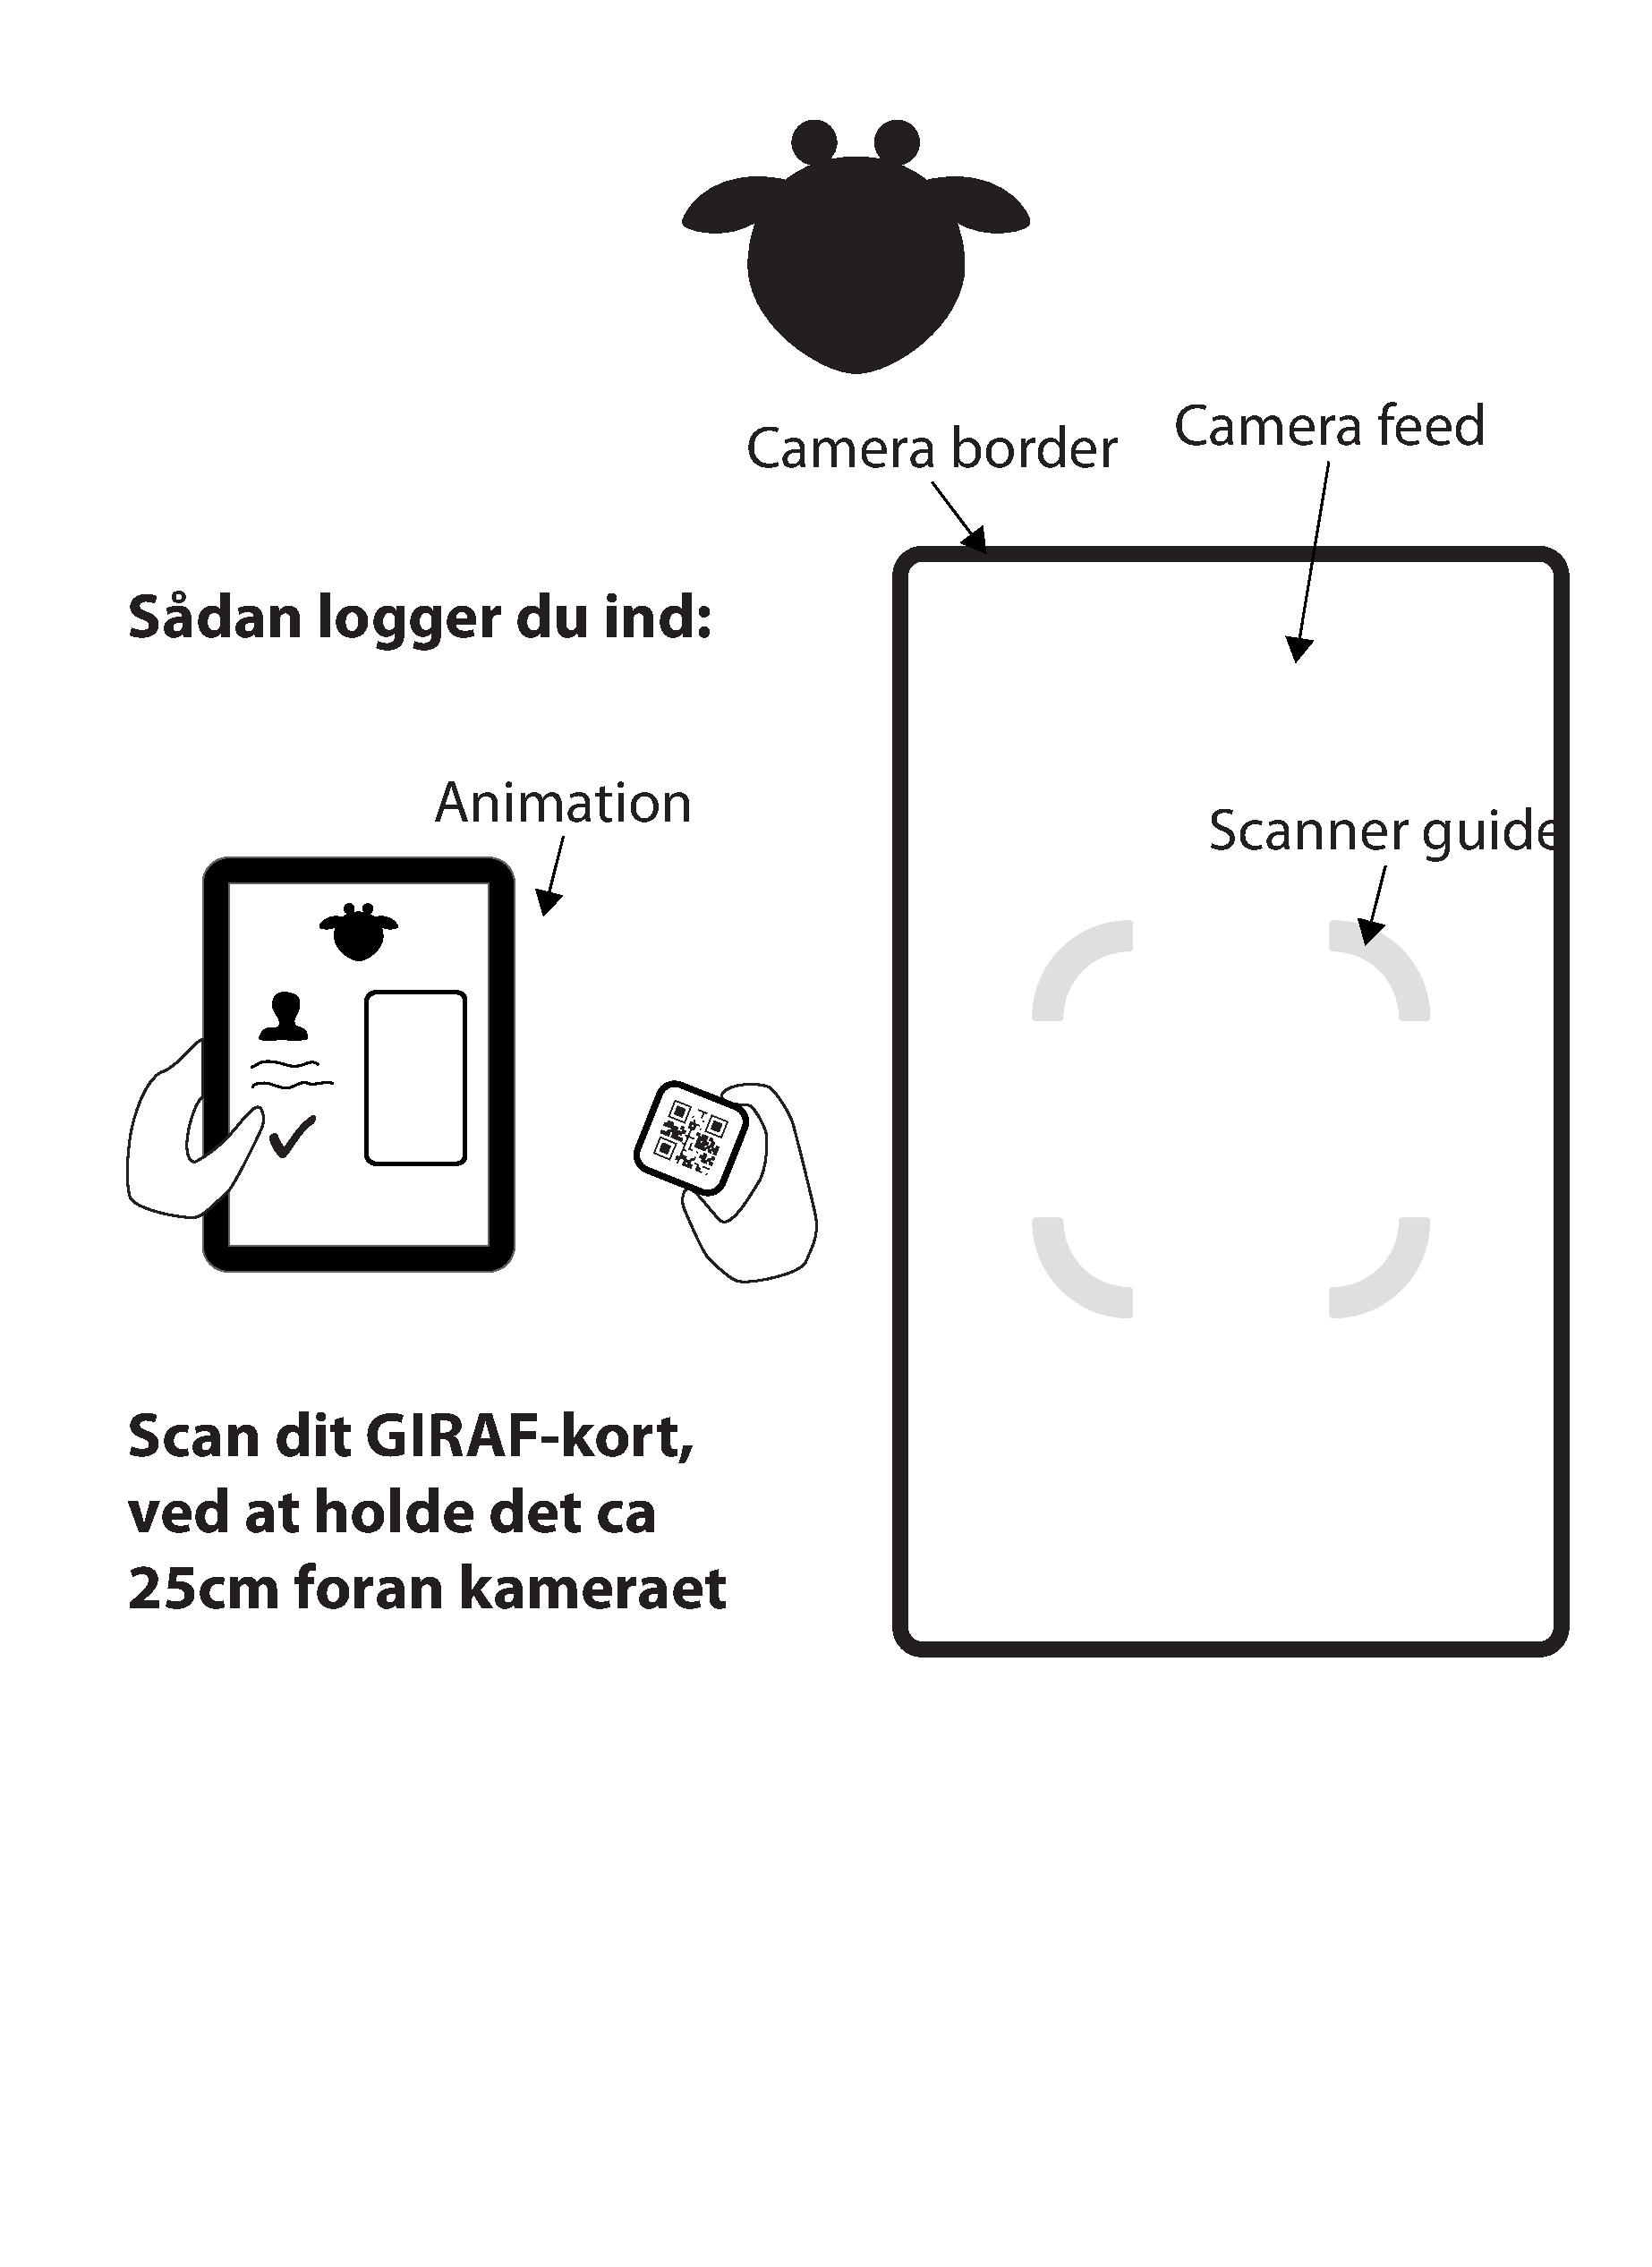
\includegraphics[width=0.7\textwidth]{gfx/authentication_bw_gui.pdf}
	\caption{Illustration of the authentication components}
	\label{fig:authentication_gui_illustration}
\end{figure}

The camera border helps distinct the camera feed from the rest of the layout, but it also provides feedback upon scanning by changing colors --- this can be seen in \autoref{app:design:authentication}. 
The backwards facing camera feed is surrounded by the camera border. 
A scanner guide is overlaid on top of the camera feed to remind the user of scanners in general and the behavior that is expected of them.
\autoref{fig:authentication_gui_design_init} shows the complete graphical design.

\begin{figure}[!h]
	\centering
	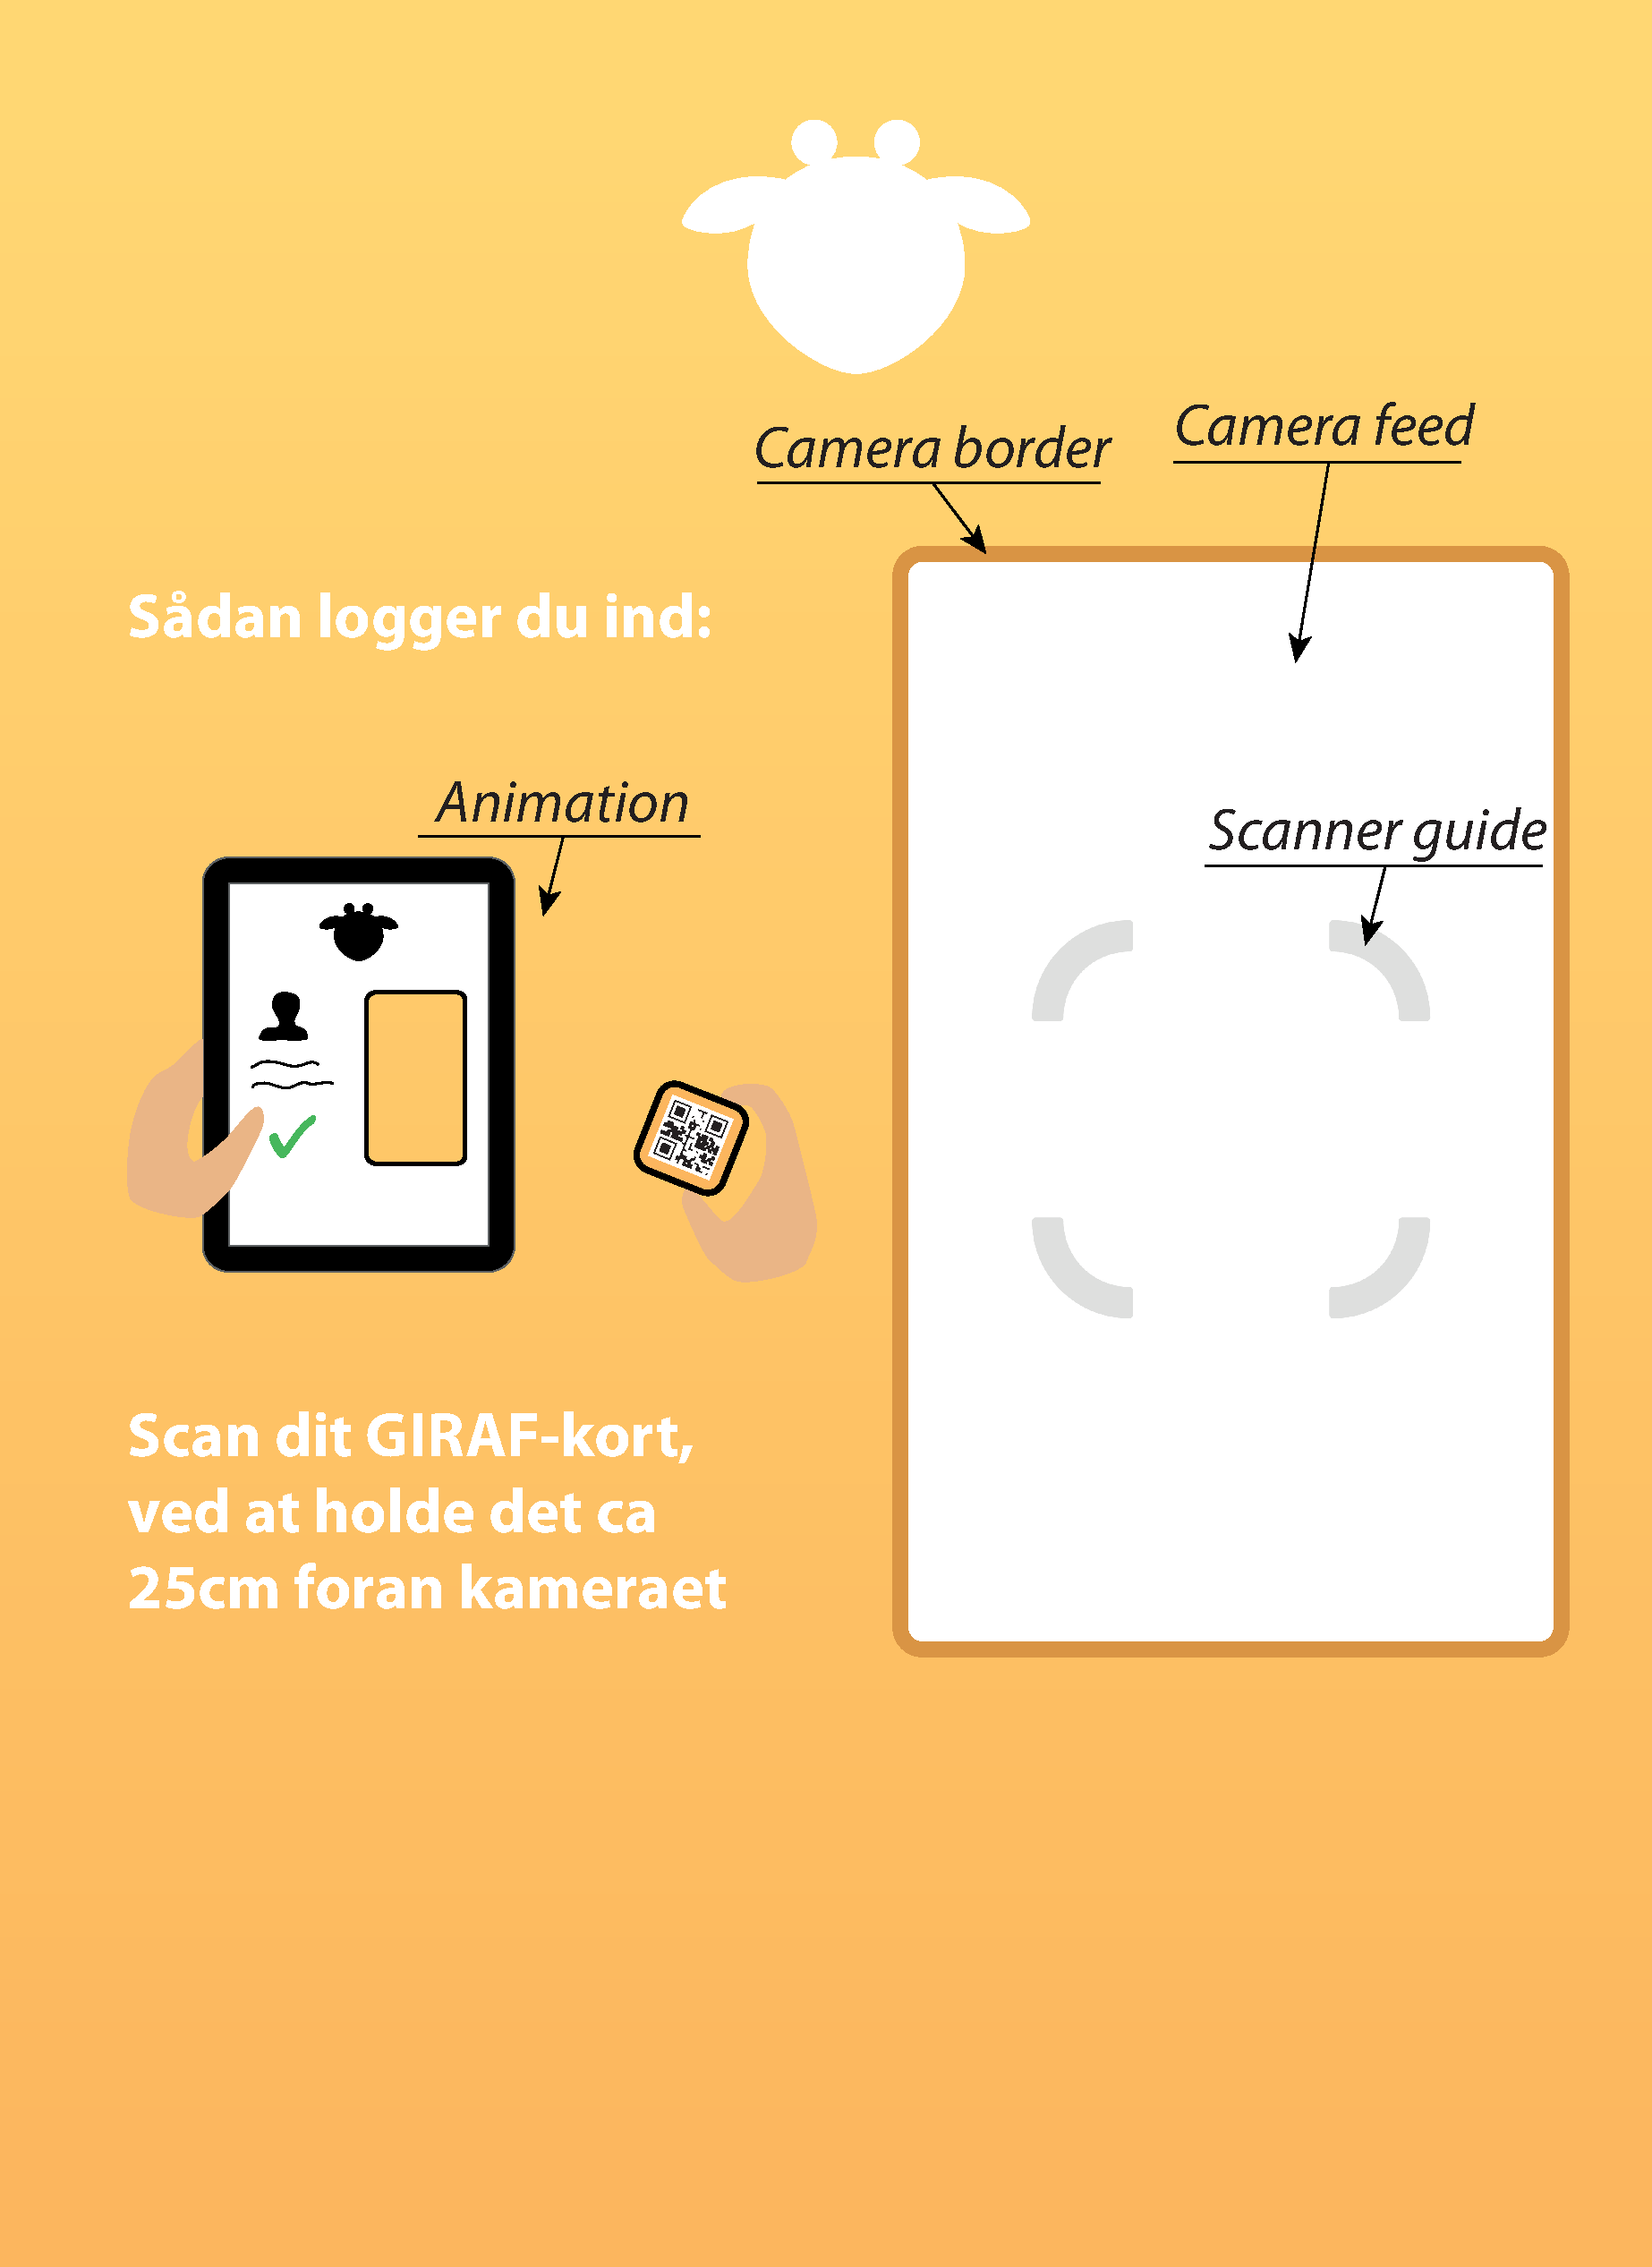
\includegraphics[width=0.7\textwidth]{gfx/authentication_gui_design_init.pdf}
	\caption{GUI of the authentication functionality}
	\label{fig:authentication_gui_design_init}
\end{figure}

On the left hand side an animation is shown, to guide the user through the scanning process. 